\documentclass{beamer}

\usetheme{Warsaw}

\usepackage[utf8]{inputenc}
\usepackage[frenchb]{babel}
\usepackage[T1]{fontenc}
\usepackage{amsmath}
\usepackage{hyperref}
\usepackage{tikz}
\usepackage{tikz-qtree}
\usepackage{graphicx}
\usepackage{listings}
\usepackage{xcolor}
\usepackage{textcomp}
%\usepackage{multicol}
\definecolor{darkgreen}{rgb}{0, 0.6, 0}

\usetikzlibrary{arrows}


\pdfcompresslevel0

\usepackage{color}

\addtobeamertemplate{footline}{\hfill\insertframenumber/\inserttotalframenumber
\hspace{10em}\\}

\usepackage{listings}

\title{HyperLogLog: Analysis and implementation of an improved algorithm}
\author{Chloé Dequeker, Ghiles Ziat}
\date{13 fevrier 2015}

% slides number
\defbeamertemplate*{footline}{shadow theme}
{%
  \leavevmode%
  \hbox{\begin{beamercolorbox}[wd=.5\paperwidth,ht=2.5ex,dp=1.125ex,leftskip=.3cm plus1fil,rightskip=.3cm]{author in head/foot}%
    \usebeamerfont{author in head/foot}\insertframenumber\,/\,\inserttotalframenumber\hfill
  \end{beamercolorbox}%
  \begin{beamercolorbox}[wd=.5\paperwidth,ht=2.5ex,dp=1.125ex,leftskip=.3cm,rightskip=.3cm plus1fil]{}%
    \usebeamerfont{title in head/foot}\insertshorttitle%
  \end{beamercolorbox}}%
  \vskip0pt%
}


\begin{document}

\maketitle

\begin{frame}{Introduction}
 Cardinality estimation problem:
  \begin{itemize}
    \item The naive solution does not scale!
    \item Several alogorithms have been proposed
  \end{itemize}

  \bigskip
  Today, we'll talk about:
  \begin{block}{HyperLogLog++ (call it HyperGoogle)}
    Improvement of the HyperLogLog
  \end{block}

\end{frame}

\begin{frame}{Hyperloglog}
  The approach of the HyperLogLog:
  \begin{itemize}
    \item Randomization using a hash function
    \item Observation of the maximum of the number of leading zeros
    \item Stochastic averaging
  \end{itemize}
  \bigskip
  The result is then subjected to corrections
  \begin{itemize}
    \item Small range correction 
    \item Large range correction
  \end{itemize}
\end{frame}

\begin{frame}{Bias estimation and correction}
  Transition to 64 bits $ \rightarrow $ an increase of the efficiency area
   
  \bigskip

  \begin{block}{Bias}
    The observed bias depends on the cardinality estimated.
    A correction then can be computed 
  \end{block} 
  
  \begin{itemize}
    \item Bias estimation
    \item Store them into a file
    \item File loading
    \item Linear interpolation
  \end{itemize}
\end{frame}

\begin{frame}
\frametitle{Memory optimization}
	\begin{itemize}
		\item How to use the least memory possible
		\item Different kinds of optimization
		\item Depending on the number of values we want to stock
		\item We use a bitmap
	\end{itemize}
	\begin{block}{Three type of representation}
		\begin{itemize}
			\item Dense representation
			\item Sparse representation
			\item Delta varint encoding : use the sparse representation
		\end{itemize}
	\end{block}
\end{frame}

\begin{frame}
\frametitle{Dense representation}
	\begin{center}
		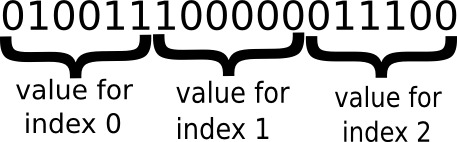
\includegraphics[width=5cm]{dense.png} \\
	\end{center}
	\begin{block}{Pros}
		\begin{itemize}
			\item Use the least possible amount of bits per value
			\item No index is stocked
			\item easy to access data
			\item Memory size of the bitmap constant
		\end{itemize}
	\end{block}
	
	\begin{block}{Cons}
		\begin{itemize}
			\item When only few items are added, takes a lot of unnecessary space
			\item When checking for empty indexes, the whole bitmap needs to be read
		\end{itemize}
	\end{block}
\end{frame}

\begin{frame}
\frametitle{Sparse representation}
	\begin{center}
		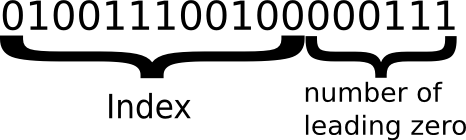
\includegraphics[width=5cm]{sparse.png} \\
	\end{center}
	\begin{block}{Pros}
		\begin{itemize}
			\item Size of the map will fit the number of values we have
		\end{itemize}
	\end{block}
	
	\begin{block}{Cons}
		\begin{itemize}
			\item It needs to stock the index AND the value
			\item Results in 20 bits for P = 14 and int 64
		\end{itemize}
	\end{block}
\end{frame}

\begin{frame}
\frametitle{Delta varint encoder and decoder}
	\begin{center}
		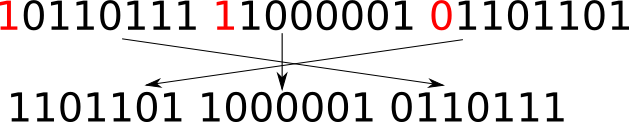
\includegraphics[width=7cm]{varint.png} \\
	\end{center}
	
	\begin{block}{Principles}
		\begin{itemize}
			\item Improves the sparse representation
			\item Will use the difference between current value and previous one
			\item It is used in order to decrease the sparse size
		\end{itemize}
	\end{block}
\end{frame}

\begin{frame}
	\begin{center}
		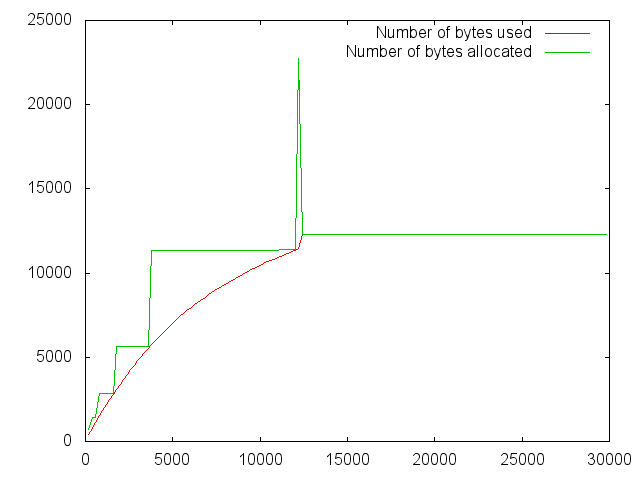
\includegraphics[width=10cm]{plot_memoryUsage.png} \\
	\end{center}
	Number of bytes used and allocated by our bitmap in function of the number of addItem() calls
\end{frame}

\begin{frame}{Conclusion}
  \begin{itemize}
    \item We implemented it
    \pause
    \item Entirely (Except for P=25)
    \pause
    \item Using \textbf{C} (best language ever)
    \pause
    \item \textbf{C99} would have been better 
    \pause
    \item It works!
    \pause 
  \end{itemize}
\end{frame}


\begin{frame}{Bibliographie}  \begin{thebibliography}{}

\bibitem{FlFuGaMeRe}
\textbf{P. Flajolet, Éric Fusy, O. Gandouet, and F. Meunier, HyperLogLog: the analysis of a near-optimalcardinality estimation algorithm}. In \emph{In Analysis of
Algorithms (AOFA)}, pages 127–146, 2007.

\bibitem{HeNuHa}
\textbf{S. Heule, M. Nunkesser, A. Hall, HyperLogLog in Practice: Algorithmic Engineering of a State of The Art Cardinality Estimation Algorithm}.

\end{thebibliography}

\end{frame}

\end{document}
